% !TEX root = ../main.tex
\section{Technical Development}

\texttt{tpeanuts} is structured as a conservative rewrite of the numerical core of PEANUTS. The implementation follows the original physical decomposition while replacing array operations by PyTorch tensors. This section describes the main components of the update.

\subsection{Software architecture}

\texttt{tpeanuts} is a PyTorch-native reimplementation of the neutrino oscillation and flux-propagation toolkit originally developed as PEANUTS (a NumPy/Numba package), extended into a full detector-level statistical-inference framework. The guiding design principle is to replace the scalar, per-point evaluation model of the original implementation with a batched, tensor-oriented formulation: every physical quantity, Hamiltonians, evolution operators, oscillation probabilities, fluxes, predicted event counts, likelihoods, is expressed as a function of broadcastable \texttt{torch.Tensor} inputs, so that large grids of energies, angles and detector configurations, within memory limits, can be evaluated in a single vectorised call. The underlying physics primitives also support automatic differentiation; the fast-forward simulation routines used for most physics results wrap them in \texttt{torch.no\_grad()} for speed, while the experiment-specific inference models of \cref{sec:inference-layer} build on the same primitives without disabling autograd, so that gradients can be backpropagated through the full chain for the gradient-based fits of \cref{sec:detector-validation-methodology}. This is the central architectural departure from both the legacy implementation and from reference tools such as \texttt{nuSQuIDS} \parencite{nuSQuIDS}, whose C++/pybind11 API is fundamentally scalar, with one solver object per energy/angle point.

\Cref{fig:modular-architecture} sketches the resulting three-tier decomposition, application, domain and core layers, detailed below. This hierarchy is itself supported by a set of blocks that sit outside it: a configuration layer centralising model choices, a shared utility layer providing standard device/precision management and generic numerical primitives, and a collection of external-tool integrations, third-party packages such as MCEq and external data repositories such as the Honda/HKKM flux tables, consumed as configuration input to the physics above rather than as part of the propagation engine itself.

\begin{figure}[htbp]
  \centering
  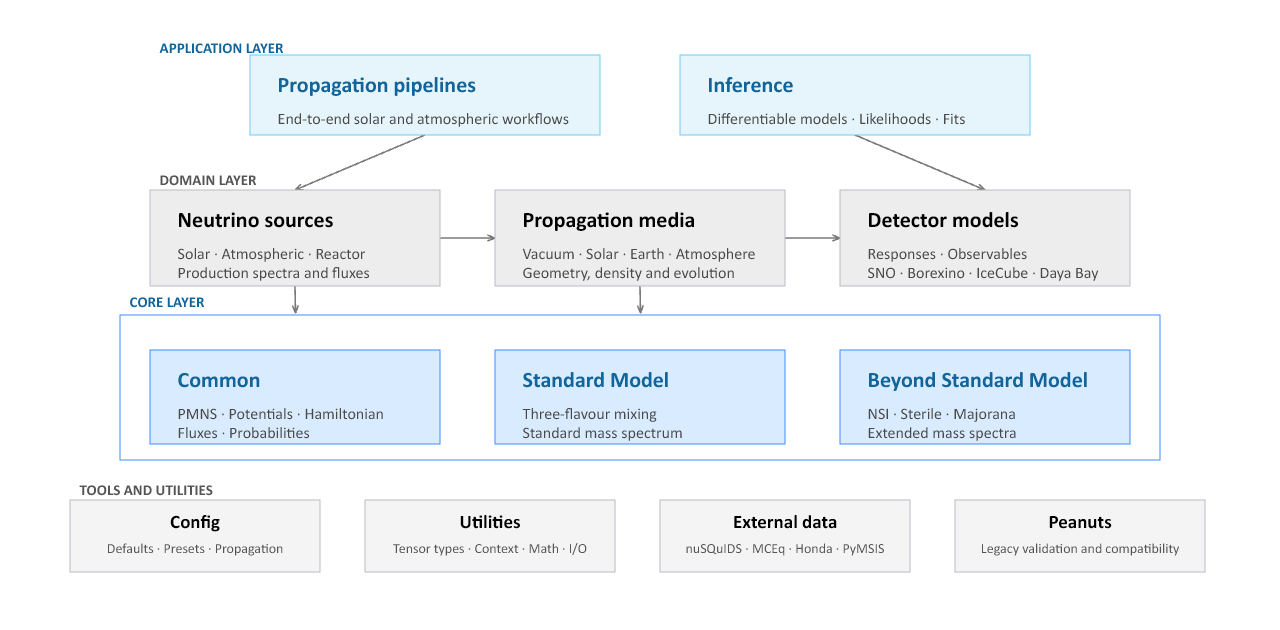
\includegraphics[width=0.9\textwidth]{figuras/desarrollo/tpeanuts_modular_architecture_diagram.png}
  \caption{Modular architecture of \texttt{tpeanuts}: an application layer (propagation pipelines, inference) built on a domain layer (neutrino sources, propagation media, detector models), which specialises a shared core (common primitives, Standard Model and BSM Hamiltonians) and is supported by configuration, utility, external-data and legacy-PEANUTS-compatibility tools.}
  \label{fig:modular-architecture}
\end{figure}

Concretely, this three-tier architecture is implemented as a set of independent Python packages, one per node of \cref{fig:modular-architecture}, summarised in \cref{tab:architecture-layers} together with the responsibility of each.

\begin{table}[htbp]
  \centering
  \footnotesize
  \caption{Packages composing \texttt{tpeanuts}, and their responsibility.}
  \label{tab:architecture-layers}
  \begin{tabularx}{\textwidth}{lX}
    \toprule
    Package & Responsibility \\
    \midrule
    \texttt{config/} & Composed configuration objects (\texttt{PropagationConfig}, \texttt{SolarParameters}) and named SM/BSM/NSI presets, replacing per-call keyword arguments. \\
    \texttt{core/} & Medium-independent Hamiltonians, PMNS/mass-spectrum construction, evolution operators; standard and BSM (\(3+1\) sterile, NSI, Majorana) variants. \\
    \texttt{source/} & Emission models at the neutrino source: solar production profiles, reactor (Huber--Mueller) antineutrino spectra. \\
    \texttt{medium/} & Environment-specific density/geometry models: vacuum, solar, Earth, atmosphere. \\
    \texttt{detector/} & Forward-folding of oscillated flux into predicted event counts: cross sections, target composition, energy response, efficiency, backgrounds, per experiment. \\
    \texttt{pipeline/} & Composition of the above into complete observables (solar/Earth/atmosphere detection chains). \\
    \texttt{external/} & Optional third-party integrations (MCEq, nuSQuIDS, Honda, PyMSIS) for cross-validation and flux/density inputs. \\
    \texttt{inference/} & Likelihood construction, gradient-based (LBFGS) fitting, Laplace/Fisher uncertainty estimation, likelihood scans. \\
    \texttt{util/} & Device/dtype management (\texttt{RuntimeContext}) and generic numerical primitives. \\
    \bottomrule
  \end{tabularx}
\end{table}

\subsubsection{Application, domain and core layers}

At the base of the hierarchy, the core layer implements the medium-independent building blocks shared by every propagation scenario, for the plain three-flavour Standard Model and for the optional BSM extensions (\(3+1\) sterile, NSI), together with an optional Majorana mass-matrix parametrisation relevant to lepton-number-violating observables rather than standard oscillation probabilities: the vacuum and matter Hamiltonians, PMNS/mass-spectrum construction, the matter potential, and the machinery to convert a Hamiltonian into a unitary evolution operator. Two complementary propagation strategies are implemented here: a perturbative/analytical evolutor for smooth, slowly varying density profiles, and a medium-independent numerical evolutor, which discretises the trajectory, exponentiates a local Hamiltonian on each segment, and composes the segment operators through a logarithmic-depth binary-tree reduction, keeping the composition fully batchable and GPU-friendly.

The domain layer specialises this shared core for each physical scenario, adding the neutrino-source, propagation-medium and detector models that the core layer itself knows nothing about. A source model isolates the physics of neutrino \emph{emission}, upstream of propagation: solar production distributions from the Standard Solar Model, and the per-isotope Huber--Mueller \parencite{Huber2011,Mueller2011} reactor-antineutrino emission spectrum. A propagation-medium model then specialises the core with an environment-specific density/geometry treatment: vacuum, solar (adiabatic MSW/Landau--Zener mixing with production-point-averaged fluxes), Earth (matter regeneration along nadir-angle trajectories, with exposure time-averaged over the detector's latitude and the Earth's rotation), and atmosphere (propagation from a production height through the atmosphere and, optionally, into the Earth).

\label{sec:detector-layer}
Finally, a detector model folds an oscillated flux into a predicted, binned event count observable, entirely decoupled from how the probability was computed: a target composition, an energy response, an efficiency and a background, common to every experiment, combined with the relevant cross section by physical process rather than by detector, inverse beta decay to order \(1/M\) \parencite{VogelBeacom1999} (reactor antineutrinos), neutrino--electron elastic scattering (solar), and deuteron dissociation (SNO). Five experiment-specific modules specialise this for Borexino, Daya Bay, IceCube DeepCore, and SNO phases~I and~II, summarised in \cref{tab:detector-experiments} and, for Daya Bay, detailed in \cref{sec:dayabay-case-study}.

At the top of the hierarchy, the application layer composes the models of the domain layer into complete, physically meaningful results. On one side, propagation pipelines assemble the source, medium and detector models into end-to-end observables, a solar-production-to-Earth-detection chain, or a full atmospheric flux propagated through the Earth; a legacy adapter over the original PEANUTS implementation is retained in full as the behavioural reference for the function-by-function translation regression check, an independent statement of physical correctness instead being established by the analytic limits and \texttt{nuSQuIDS} comparisons of \cref{sec:validation-strategy}.

\label{sec:inference-layer}
On the other side, built on the same validated primitives, the statistical-inference machinery implements the formalism of \cref{sec:inference-formalism} as reusable, detector-agnostic components: a common differentiable-model interface, a free-parameter tuple and a prediction function, that every concrete model, oscillation-only or detector-composed, implements; a set of likelihood functions covering Poisson counts, asymmetric Gaussian ratios and, for covariance-matrix observables such as SNO~II's 38-observable data set, a correlated Gaussian likelihood, together with a Gaussian penalty term for externally constrained nuisance parameters; an LBFGS minimiser paired with the Laplace/Fisher covariance estimate; and a two-dimensional likelihood-scan routine, with an optional per-point re-minimisation of the remaining free parameters. The concrete, experiment-specific models composing an oscillation model with a detector's event-rate function live alongside each detector.

\subsubsection{External-tool integrations (\texttt{external/})}

This layer isolates optional third-party dependencies from the core physics code: \texttt{external/mceq/} wraps the MCEq cascade-equation solver \parencite{Fedynitch2015}; \texttt{external/nusquids/} wraps \texttt{nuSQuIDS} \parencite{nuSQuIDS} as an independent reference for validation and benchmarking; \texttt{external/honda/} reads the Honda/HKKM atmospheric-flux tables \parencite{Honda2007}; \texttt{external/pymsis/} provides an empirically calibrated atmospheric density model \parencite{Emmert2021}. Each is imported lazily so the package degrades gracefully when the optional extras are not installed.

\begin{table}[htbp]
  \centering
  \footnotesize
  \caption{Experiments implemented on the detector/inference layers, and their validation status against real published data (\cref{sec:other-experiments}).}
  \label{tab:detector-experiments}
  \begin{tabularx}{\textwidth}{lXX}
    \toprule
    Experiment & Channel / detector physics & Status against real data \\
    \midrule
    Daya Bay & Reactor \(\bar\nu_e\) IBD, 8 detectors, 6 reactors, full flux/response chain & Near/far fit recovers \(\sin^22\theta_{13}\), \(\Delta m^2_{31}\) jointly within 1--2\% of published (\cref{sec:dayabay-case-study}); full-shape fit not yet robust \\
    IceCube DeepCore & Atmospheric \(\nu_\mu\) disappearance, event-by-event weighted-MC reweighting & Fit recovers \(\theta_{23}\), \(\Delta m^2_{3l}\) within \(-0.05\sigma\) of published; fitted muon-background normalisation traced to fixed detector systematics \\
    SNO~II (salt phase) & CC/NC/ES, 38 published observables, published statistical covariance plus a reconstructed systematic covariance (NC's own dedicated systematics not yet transcribed) & Fit converges to \(\theta_{12}\), \(\Delta m^2_{21}\), \(\lambda_{8B}\) consistent with SNO's own SNO-only range; Laplace uncertainty on \(\Delta m^2_{21}\) breaks down once the reconstructed covariance is included, motivating the likelihood-scan machinery \\
    Borexino & Solar \(\nu\)--\(e\) elastic scattering, pp-chain spectrum & Detector response and event-rate chain implemented; background model and energy-resolution normalisation not yet taken from the published analysis \\
    SNO (phase~I) & CC/NC/ES, pure-D\(_2\)O phase & Cross sections, response and inference model implemented and unit-tested; not yet exercised against a full published data set \\
    \bottomrule
  \end{tabularx}
\end{table}

\subsubsection{Notebooks: validation, benchmarking, analysis, reproduction and inference}

Beyond the architecture described above, a curated suite of notebooks exercises every layer of \texttt{tpeanuts} and constitutes the primary, reproducible evidence base behind every result reported in this thesis. The suite is organised into four complementary groups.

\begin{itemize}
  \item \textbf{Validation and benchmark} notebooks establish bit-level agreement against legacy PEANUTS and cross-validate against \texttt{nuSQuIDS} for every propagation medium (\cref{sec:validation-strategy}), and measure CPU/GPU performance against both references (\cref{sec:benchmarking-methodology}).
  \item \textbf{Solar and atmospheric analysis} notebooks explore the fundamentals of each propagation regime, production and exposure profiles, differential-flux structure, and the behaviour of the underlying density models, independently of any specific detector or experiment.
  \item \textbf{Reproduction} notebooks recover well-known physical signatures, the solar day--night asymmetry, the MSW resonance, atmospheric oscillograms, Earth matter tomography, and the LMA-Dark degeneracy, establishing that the implementation reproduces established physics independently of any single reference code (\cref{sec:extension-methodology,sec:bsm-methodology}).
  \item \textbf{Inference} notebooks close the chain, running real-data prediction checks, normalisation audits and parameter-recovery fits where the experimental model is sufficiently complete (Daya Bay, IceCube DeepCore and SNO phase~II); Borexino and SNO phase~I are currently validated only at component and unit-test level (\cref{sec:detector-validation-methodology}).
\end{itemize}

The full notebook directory tree is given in \cref{sec:supplementary-material}.

\subsection{Numerical simulation conventions}

The numerical core of \texttt{tpeanuts} is built around a small number of deliberate conventions that keep every propagation medium numerically consistent, dimensionally well-behaved, and directly comparable to both the legacy PEANUTS implementation and to \texttt{nuSQuIDS}. The most important of these are the choice of a unitary, dimensionless evolution scale for the Hamiltonian, the neutrino/antineutrino sign convention, and the floating-point precision policy used throughout the matrix-exponential evolution.

\subsubsection{Non-dimensionalisation of the Hamiltonian}

Rather than working directly with the physical matter potential and kinetic (mass-squared) terms, which span many orders of magnitude depending on the neutrino energy and the medium's density, every Hamiltonian contribution is first converted into a dimensionless quantity by multiplying it by a configurable evolution length scale, \texttt{evolution\_scale\_m} (the Earth radius, by default). Concretely,

\begin{equation}
  V = s\,L_{\mathrm{scale}}\sqrt{2}\,G_F\,N_A\,\bigl(10^{6}\,\mathrm{cm^3/m^3}\bigr)\,(\hbar c)^2\,n_e,
  \qquad
  k_i = L_{\mathrm{scale}}\,\frac{\Delta m_i^2}{2E\hbar c},
\end{equation}

where \(s=\pm1\) is the neutrino/antineutrino sign (see below), \(N_A\) is Avogadro's number and the \(10^6\,\mathrm{cm^3/m^3}\) factor converts \(n_e\), the electron number density in \(\mathrm{mol/cm^3}\), to \(\mathrm{mol/m^3}\) consistently with \(L_{\mathrm{scale}}\) in metres, and \(\Delta m_i^2\) are the (reduced) mass-squared eigenvalues. The trajectory coordinate is normalised by the same scale, \(x=L/L_{\mathrm{scale}}\), so that the evolution operator is always computed as \(U=\exp(-iHx)\), with both \(H\) and \(x\) dimensionless.

This convention has two practical benefits for a batched, GPU-oriented implementation: it gives a uniform dimensionless convention for every propagation medium, avoiding mixed physical length units inside the evolutors, without changing the physical phase \(\hat Hx=H_{\mathrm{phys}}L\) or the matrix argument passed to the exponential; and it decouples the physical unit system from the propagation length, since only the ratio \(L/L_{\mathrm{scale}}\) ever enters the exponent. The evolution scale defaults to the Earth's radius for backward compatibility with the legacy PEANUTS convention, but is an explicit, per-medium parameter, settable e.g.\ to the injection height of an atmospheric shower rather than to \(R_\oplus\).

\subsubsection{Neutrino/antineutrino convention}
\label{sec:antinu-convention}

Antineutrino propagation is selected through a single boolean (or boolean-tensor, for batched mixed samples) flag, \texttt{antinu}, carried by the \texttt{OscillationParameters} object and threaded through every Hamiltonian and probability routine. Two independent sign flips are applied consistently whenever \texttt{antinu=True}:

\begin{itemize}
  \item \textbf{Matter potential.} The Wolfenstein charged-current potential changes sign, \(V\to-V\), since it originates from the coupling of \(\nu_e\) (not \(\bar\nu_e\)) to the ambient electrons.
  \item \textbf{Mixing matrix.} The PMNS matrix is replaced by its complex conjugate, \(U\to U^{*}\), equivalent to flipping the sign of the CP-violating phase, \(\delta_{\mathrm{CP}}\to-\delta_{\mathrm{CP}}\).
\end{itemize}

Both substitutions are applied at the point where the reduced mixing matrix and the matter Hamiltonian are assembled, so that every downstream propagation routine, vacuum, solar, Earth or atmospheric, inherits the correct antineutrino behaviour automatically from a single flag, without medium-specific antineutrino logic. The same object also encodes the neutrino mass ordering as the sign of the atmospheric splitting \(\Delta m^2_{3l}\): a positive value selects normal ordering and a negative value selects inverted ordering, both handled by a single \texttt{torch.where} branch, so that mixed-ordering batches (e.g.\ for an ordering-marginalised analysis) can, in principle, be evaluated in one call.

\subsubsection{Precision and evaluation mode}
\label{sec:precision-modes}

All propagation is carried out at double precision (\texttt{torch.float64} real / \texttt{torch.complex128} complex) by default, matching the precision of the legacy NumPy implementation and keeping the matrix-exponential composition numerically stable over trajectories segmented into hundreds of steps. The fast-forward simulation pipelines are wrapped in \texttt{@torch.no\_grad()} by default, since most forward evaluation, benchmarking and physics reproduction does not need gradients and disabling autograd bookkeeping reduces memory footprint and computational overhead; the underlying physics primitives themselves, and the experiment-specific inference models built directly on them (\cref{sec:inference-layer}), do not disable autograd, and it is this differentiable path, not the fast pipelines, that drives the gradient-based fitting of \cref{sec:detector-validation-methodology}.

For validation purposes, a \texttt{legacy\_precision} flag is threaded through the potential and Hamiltonian builders; when enabled, it substitutes the full-precision matter-potential prefactor, derived from CODATA \(G_F\), \(N_A\) and \(\hbar c\) \parencite{CODATA2021}, with the four-significant-digit constant hard-coded in the original PEANUTS implementation, allowing bit-level, rather than merely physics-level, agreement to be verified against the legacy reference where required.

\subsection{Neutrino detection pipelines}
\label{sec:pipelines}

Beyond the medium-specific propagation primitives described above, the framework assembles them into two complete, physically distinct detection workflows: a solar-neutrino pipeline, which propagates neutrinos produced deep inside the Sun to a terrestrial detector, and an atmospheric-neutrino pipeline, which propagates neutrinos produced by cosmic-ray air showers in the Earth's atmosphere down to a detector. Both share the same underlying core Hamiltonian/evolutor machinery, but differ fundamentally in one respect: whether the mass-eigenstate coherence acquired at production survives all the way to the detector.

\subsubsection{Solar-neutrino detection pipeline}

A solar neutrino is produced as a pure \(\nu_e\) at some radius \(\rho\) inside the Sun, distributed according to a source-specific production profile (e.g.\ \({}^8\mathrm{B}\), \(pp\)) \parencite{Vinyoles2017}. As it propagates outward through the Sun's smoothly varying electron density, the MSW matter effect adiabatically rotates the flavour state into the local mass-eigenstate basis, with a small non-adiabatic level-crossing correction \parencite{Parke1986}. Because the \(\sim1.5\times10^{8}\,\mathrm{km}\) vacuum baseline to Earth is enormously larger than the oscillation length at solar-neutrino energies, the relative phases between mass eigenstates wash out completely before arrival: only the incoherent mass-eigenstate populations survive.

\texttt{tpeanuts} implements this picture as a pipeline reproducing, in batched \texttt{torch} form, the original PEANUTS NumPy/Numba reference workflow used to validate it bit-for-bit. The pipeline proceeds in three stages:

\begin{enumerate}
  \item \textbf{Solar production and adiabatic conversion}: for a given source and energy grid, the electron-neutrino state is propagated adiabatically outward from each production radius \(\rho\) in the source's normalised production-radius distribution, and the result is averaged over that distribution to yield a single vector of mass-eigenstate weights, \(w_i(E)=(w_1,w_2,w_3)\), the fraction of the flux exiting the Sun in each mass eigenstate.
  \item \textbf{Vacuum propagation to Earth}: because no relative phase is ever tracked, propagation across the Sun--Earth vacuum baseline leaves the mass weights \(w_i(E)\) unchanged by construction; this step is a physical no-op in the incoherent formulation, not an approximation applied afterwards.
  \item \textbf{Earth matter propagation}: at the detector, the incoherent mixture of incident mass eigenstates is propagated through Earth matter, relevant only for underground detectors sensitive to the day/night matter-regeneration asymmetry, evaluated over a grid of nadir angles \(\eta\); each mass eigenstate acquires its own Earth-matter transition probability to each final flavour \(\alpha\), \(P^\oplus_{i\to\alpha}(E,\eta)\), and the final flavour probability is their incoherent sum, \(P_{\nu_e\to\nu_\alpha}(E,\eta)=\sum_i w_i(E)\,P^\oplus_{i\to\alpha}(E,\eta)\).
\end{enumerate}

This oscillation probability, still a function of energy rather than a detector observable, is further averaged: over the solar production-radius distribution (folded into the first stage), over the neutrino energy spectrum, and, for underground detectors, over the detector's nadir-angle exposure, the fraction of a year during which each nadir angle is observed, computed from the detector's geographic latitude and the Earth's daily and annual motion; converting it into a predicted event rate additionally requires the flux, cross section and detector response of \cref{sec:detector-layer}.

\subsubsection{Atmospheric-neutrino detection pipeline}

Atmospheric neutrinos follow a different physical picture. They are produced not at a single well-defined point but across a broad, energy- and angle-dependent distribution of production heights \(h\) in the atmosphere, with the boundary-condition flux \(\Phi_\beta(E,h,\theta)\) for each produced flavour \(\beta\) supplied by an external cascade-equation generator (MCEq \parencite{Fedynitch2015}) or by tabulated Honda/HKKM fluxes \parencite{Honda2007}, which provide \(\nu_e\), \(\bar\nu_e\), \(\nu_\mu\) and \(\bar\nu_\mu\); the negligible conventional \(\nu_\tau\) flux is carried with zero initial value. Unlike the solar case, coherence is not lost here: even for an upward-going, Earth-crossing trajectory of up to \(\sim1.3\times10^4\,\mathrm{km}\) (\cref{sec:propagation-fundamentals}), the mass-eigenstate wave packets remain overlapped at these energies and detector resolutions, so the full flavour-amplitude state is propagated coherently from production to detector. The pipeline proceeds in five stages:

\begin{enumerate}
  \item \textbf{Flux selection}: one produced particle and one detector zenith angle are sliced out of the loaded height/energy/angle flux dataset.
  \item \textbf{Atmosphere propagation}: a coherent unit-amplitude flavour state \(\ket{\beta}\) is evolved from each production height down to the Earth's surface, batched jointly over the full energy \(\times\) height grid.
  \item \textbf{Earth propagation}: for an upward-going, Earth-crossing trajectory, the surface state is propagated further through Earth matter to the detector depth, using the same coherent evolutor as the solar pipeline's coherent variant.
  \item \textbf{Height integration}: the detector-level flux for each final flavour \(\alpha\) is obtained by weighting the propagated \(\beta\to\alpha\) probability at each height by \(\Phi_\beta(E,h,\theta)\) and trapezoidally integrating over \(h\).
  \item \textbf{Flavour summation}: the height-integrated contributions from every produced flavour (\(\nu_e,\nu_\mu,\nu_\tau\) and antiparticles) are summed into the total detector-level flux of each final flavour.
\end{enumerate}

\subsection{Test suite and sanity checks}

Correctness in \texttt{tpeanuts} is established through a dedicated automated test suite of 942 test functions organised into 64 files that mirror the package's module tree one-to-one, extended with new test directories for the detector and inference layers as they were built. The suite is executed manually with \texttt{pytest} after relevant modifications, and falls into four broad, partly overlapping categories, complemented by a further, notebook-level layer of validation:

\begin{itemize}
  \item \textbf{Code consistency checks} verify the software contract of each function independently of the underlying physics: output shape/dtype/device, broadcasting over batched grids, exceptions on invalid inputs, consistency between alternative code paths (e.g.\ \enquote{analytical} vs.\ \enquote{numerical}), and save/load round-trips. This is the largest category, roughly a third to two-fifths of the suite.
  \item \textbf{Mathematical checks} verify that a function's output matches an independently derived closed-form expression or exact algebraic identity: the PMNS matrix's unit-modulus determinant and Jarlskog invariant; the composed segment-evolutor product against a manually accumulated matrix product; agreement between the perturbative and purely numerical evolutors on a constant-density segment; a resonance radius against its closed-form solution; and every non-dimensionalised term against its defining formula under parameter scaling. Roughly a quarter to a third of the suite.
  \item \textbf{Physical coherence checks} verify that computed quantities respect the physical constraints of the theory, independently of how they were computed: probability conservation (every complete, \(N\)-flavour unitary-evolution transition matrix doubly stochastic); unitarity of every evolution operator; recovery of known physical limits (zero baseline/density reduces to the identity, the adiabatic solar limit as the Landau--Zener probability vanishes, the expected antineutrino day/night asymmetry direction); and, most stringently, function-by-function cross-validation against the original PEANUTS NumPy/Numba reference. Roughly a third to two-fifths of the suite.
  \item \textbf{Detector and inference validation}: because these layers have no independent reference implementation to compare against, their unit-test coverage focuses on code-consistency and mathematical checks instead, e.g.\ the invertibility of the Daya Bay experimental model's \((\theta_{13},\Delta m^2_{31})\leftrightarrow(\sin^22\theta_{13},\Delta m^2_{ee})\) reparametrisation on its restricted physical branch, or that the IAV$\to$LSNL$\to$Gaussian-resolution response composition conserves total probability; the physical-coherence role played elsewhere by comparison with PEANUTS/\texttt{nuSQuIDS} is instead played by the closure tests and parameter-recovery fits of \cref{sec:detector-validation-methodology}, run as notebooks rather than automated test cases.
  \item \textbf{Notebook-level validation}: beyond the automated test suite, a second, complementary layer of validation lives in a dedicated set of notebooks, which reproduce bit-level agreement against legacy PEANUTS via \texttt{legacy\_precision} and cross-check against \texttt{nuSQuIDS} \parencite{nuSQuIDS} within scenario-dependent tolerances, machine precision for vacuum and atmospheric propagation, percent-to-ten-percent-level for solar and solar-Earth-detection observables (\cref{sec:validation-strategy}), for every propagation medium; run real-data prediction checks and, where the detector model is sufficiently complete, the normalisation audits and parameter-recovery fits of \cref{sec:detector-validation-methodology}; and embed inline \enquote{smoke test} cells, printed diagnostics followed by assertion statements, that must pass before the notebook is considered valid.
\end{itemize}
